\chapter{\cloudcast}

As has been illustrated in the introduction, many strategies aimed at
augmenting \ptop systems with \cloud entities, have been
proposed. Even though they embrace profoundly different philosophies,
a distinctive element common to all of the surveyed methods
is that the \cloud lives on a different conceptual level with respect
to the \ptop system: the two components work together to achieve the
final goal, but they are not integrated in an unified architecture.

In this respect \cloudcast \cite{Cloudcast} represents a novel approach
of \emph{peer-assisted} distributed computing, tailored for content
distribution scenarios. Indeed all the functionality of the system are
tightly bound to the \cloud: not only the actual information
dissemination, but also the entire management of the \ptop network
(including node bootstrap, membership and topology management). There is
no need for \emph{active} elastic computing instances, as the
whole design is conceived to be supported by a \emph{passive} storage
service such as \amazonsss.

Thanks to this central role of the \cloud and the way the topology is
maintained, \cloudcast is able to approximate a constant number of accesses
to the storage service independently of the network size, while
being able to scale in both directions. A small system characterized by
few users will mostly exploit the \cloud to deliver informations. As
more users join, the load will be spread on the
\ptop network. In all cases the amortized cost of the storage service
will remain under control: even better, the cost per user will
decrease as the user base increases.

\section{Architecture}
From an architectural viewpoint, \cloudcast is composed by two
well known \gossip protocols:
\peersampling \cite{GossipPeerSampling}
and \epidemic broadcast \cite{EpidemicAlgorithms}.
The former is responsible of bootstrapping and maintaining the topology,
whilst adjusting the \cloud contact rate as a function of the number
of nodes. The latter takes care of the actual information
dissemination, using the first as a source of peers, and it is in turn
divided into two instances: \antientropy and \rumormongering.

An overview of \cloudcast's architecture is shown in
Figure~\ref{fig:cloudcast-architecture}. The labeled arrows highlight the
interactions between the various components from the point of view of a
single peer.

\begin{figure}
  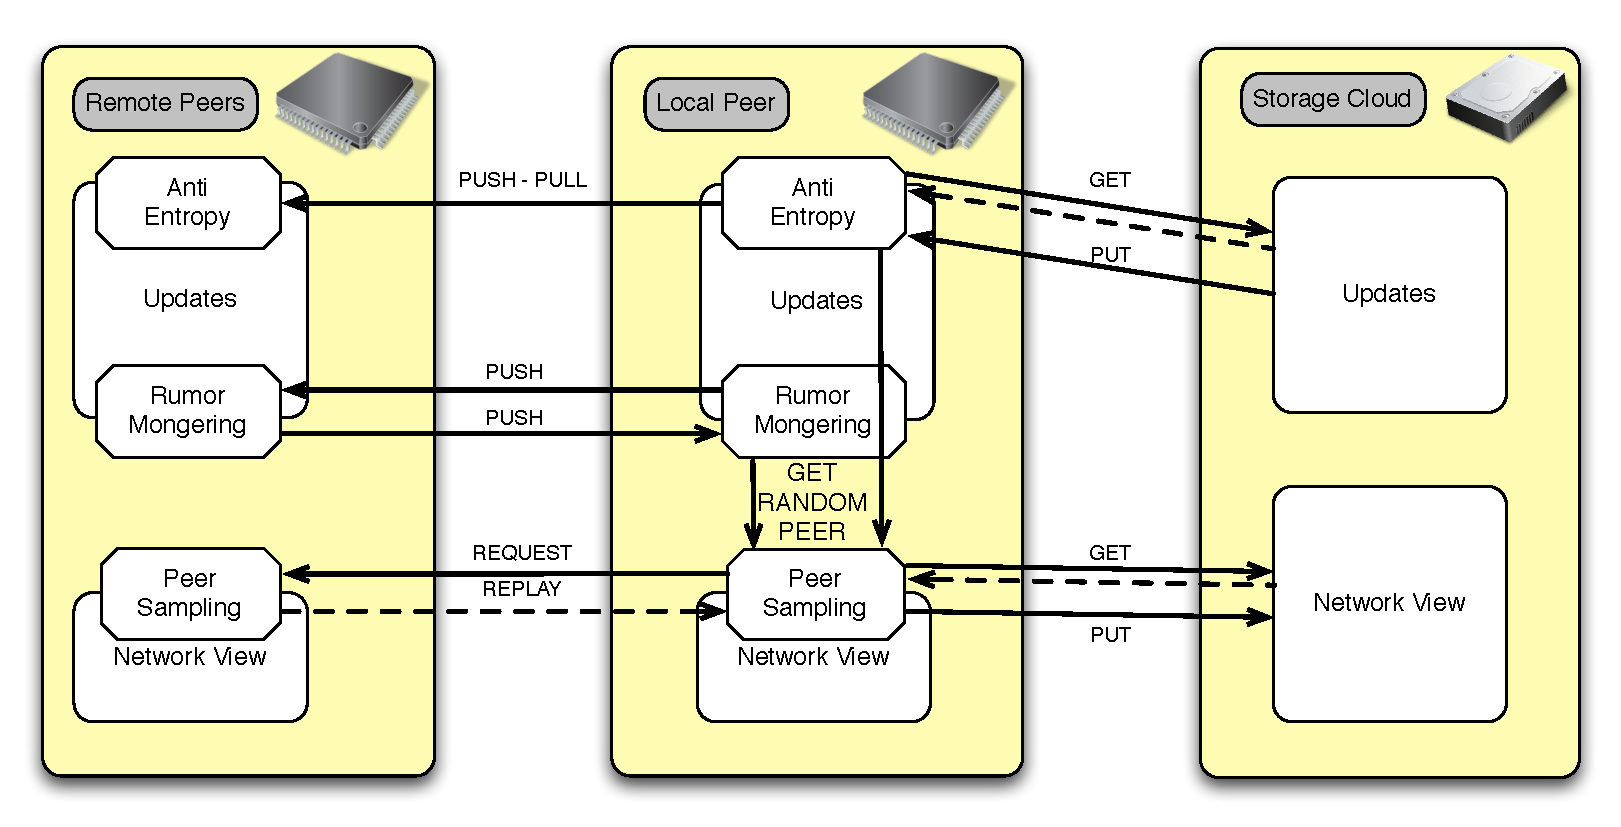
\includegraphics[width=\textwidth]{cloudcast-architecture.pdf}
  \caption{\cloudcast architecture summary highlighting component
    interactions from the point of view of a single peer}
  \label{fig:cloudcast-architecture}
\end{figure}

As can be seen, both the peers and the \cloud maintain the same set of
information (updates on information to be diffused and partial view of
the system membership): the only difference lays in the fact that the latter
lacks any active involvement.
\ \\
In the following sections we analyze in detail the protocols
forming the \cloudcast architecture with a particular focus on the
\cloud interactions.

\section{Peer Sampling}
The \peersampling protocol at the heart of \cloudcast is built upon
\cyclon \cite{CYCLON}, a well known \peersampling \gossip protocol
which has proven to provide good randomization and churn resistance,
while at the same time approximating a constant node in-degree.

In \cloudcast each node maintains a partial \view\ of the entire system
in the form of node \descriptors. Periodically each node selects
a partner to execute an information exchange, during which old
\descriptors are potentially removed (to take care of failed or
otherwise unresponsive nodes), new ones are created (to notify that the
peers involved in the exchange are still active) while existing
entries are shuffled (to satisfy the randomization property which
guarantees the network graph connectivity).

The protocol relays on a set of parameters which directly influence its
performances. Firstly the ones inherited by \cyclon: the period of
the information exchange (\deltacyclon), the size of the partial
\view\ of the network known by each peer ($c$) and the length
of the message exchanged in each cycle ($g$). Furthermore
\cloudcast introduces the variable $k$ which is used to tune the
\cloud contact frequency.

Algorithm \ref{algo:cloudcast_original_active} shows the operations
performed by the active thread of the protocol, while algorithms
\ref{algo:cloudcast_original_passive_peers} and
\ref{algo:cloudcast_original_passive_cloud} illustrate the actions
executed in response to events by the passive thread (for a clearer
explanation of the changes introduced, with respect to the original
\cyclon protocol, refer to \cite{Cloudcast}).

% Insert original cloudcast's protocol algorithms
\input algorithms/cloudcast_peersampling_algo

Every \deltacyclon\ each node fills its local \view\ by reinserting
entries sent in the previous cycle (block 1), thus
maximizing the out-degree and at the same time preventing loosing
entries (the rationale behind this statement will be evident later).
In code block 2 all the \descriptors in the \view\ are aged
by 1. Next, in block 3, the oldest \descriptor (the one with
the maximum timestamp) is selected and removed from the \view: this
has the effect of clearing the overlay from old entries associated to
failed nodes.

At this point the behavior of the protocol differs in function of the kind
of peer selected in the previous step. In case of a \cloud entry, a
request is sent to the storage service for the key ``view''
(block 4). If instead the selected partner is a normal peer,
a \request\ object containing up to $g$ \descriptors (removed from the
local \view) is created and consecutively sent to the counterpart
(block 5-6). The number of entries contained in
the \request\ is stored in the variable $res$ and has the purpose of
specifying an upper bound on the number of \descriptors expected as a
response by the remote peer.

Algorithm~\ref{algo:cloudcast_original_passive_peers} shows the actions
performed in response to peers related
events. Blocks 7-9 handle requests generated by
the active thread. Peers shuffle the local \view\ by randomly exchanging
\descriptors with the ones present in the \request\ object
and at the same time generating a \reply\ containing the removed local
entries. The $res$ variable plays an important role here: if the peer
was in the middle of an active cycle, the constraint of filling the
local \view\ for as much as $c - res$ elements would guarantee that, when
the counterpart's \reply\ will be received, there will be enough free
space to hold its content.

In block 10 it can be seen the procedure which terminates an
active cycle: peers just absorb the \reply's entries and clear the
space reservation by assigning 0 to $res$.

Up until here, apart from the minor divergence in the active
thread, the protocol closely follows \cyclon. The novelty of the
approach can be appreciated in
algorithm~\ref{algo:cloudcast_original_passive_cloud}.
Here peers simulate an entire dialogue with the \cloud (which being
a passive entity cannot take part in the protocol
itself). Block 11 and 12 emulate respectively
the construction of a local \request\ and a remote \reply. Whereas
the former is built accordingly to the previously described procedure,
the formation rules of the latter are more complex. Indeed
block 12 is the responsible for the maintenance of the
expected number of \cloud \descriptors. The \reply\ is populated with
a variable number of \cloud entries in the interval [0,2] in function
of the current contact frequency of the storage service.

To perform this adaptive scheme, \cloudcast exploits the modification
timestamp (represented by $t$ in the algorithm) associated to each
object by the storage service. If it indicates that the \cloud is not
being contacted too frequently (i.e. $now() - t >$ \deltacyclon $* k$)
then a first entry is added. Furthermore if it shows that the contact
rate is too sporadic (i.e. $now() - t >$ \deltacyclon $/ k$) then a
second entry is included.
The aforementioned parameter $k$ is adopted here to tune the time
window defining the target contact frequency: values tending towards 1
will result in an always more narrower window peaked on \deltacyclon\
(i.e. only one contact per each \cyclon cycle is acceptable) while
higher values allow more relaxed constraints.

Once the \request\ and \reply\ are completely formed they are merged
respectively with the \cloud and the local \view. This is carried out by
blocks 14 and 15. At this point the
simulated cycle is almost completed: both the \views are shuffled and new
\descriptors are added. The only remaining action to be performed by
the peer is to write the modified \view\ to the storage cloud
(block 15).

\section{Epidemic Broadcast}
\label{sec:epidemicbroadcast}
As previously mentioned, the actual information dissemination is
carried out by two \epidemic broadcast protocols. The
\antientropy instance is run periodically (every \deltaAntiEntropy)
and is responsible to
reduce differences between peers: asymptotically this guarantees that
all node receive all the updates. To fulfill this promise the
protocol have to be fairly expensive in terms of bandwidth, as it
requires the full set of data to be exchanged by involved
peers. Having to take into account the \cloud alongside standard peers,
the original algorithm by Demers~\cite{EpidemicAlgorithms} must be
adapted to the current scenario:
algorithm~\ref{algo:cloudcast_antietropy} shows the modified pseudo
code.
In block (ae1) the \cloudcast \peersampling protocol is queried
for a random peer currently in the \view. Blocks (ae3) and (ae4)
implement the original difference resolution between peers, while
block (ae2) adds the interaction with the \cloud.
All the strategies discussed in the paper are supported by
\cloudcast and are reflected in the code by the parameter
\emph{strategy}.

% Insert anti entropy protocol
\input algorithms/cloudcast_antientropy_algo.tex

Having solved the problem of comprehensively diffuse updates, the last
protocol in the architecture deals with the complementary task of
quickly and efficiently distribute updates in a \emph{reactive} fashion. This is the
role played by the \rumormongering \epidemic broadcast.
In \rumormongering, peers are initially \emph{ignorant}. Whenever they
receive an update this becomes an \emph{hot-rumor}. Peers holding an
\emph{hot-rumor}
select, every \deltaRumorMongering time units, a random peer in the current
topology and send (\emph{push}) the update to it. The rumor ceases to
be hot according to different strategies~\cite{EpidemicAlgorithms},
 all of which are applicable with \cloudcast.
As can be seen in figure~\ref{fig:cloudcast-architecture}, \rumormongering\
does not interact directly with the \cloud, but involves only normal
peers.

The rationale behind this choice is that, by its very nature, the
protocol is \emph{reactive} and hence not applicable to a
\emph{passive} entity. Furthermore \cloud \descriptors are
excluded from the random selection of peers to avoid that the
introduction of an update results in an \emph{explosion} of contacts
to the storage service. This does not affect the quality of the
information dissemination, as the \cloud will in any case receive the
news thanks to the \antientropy instance.

The algorithm for this protocol is omitted, as it does not need any
modification to be adopted in \cloudcast; for more information on the
implementation refer to the original paper\cite{EpidemicAlgorithms}.

\section{Simulation results}
\cloudcast has been subjected to many simulations performed with the event
driven version of the \textit{PeerSim P2P Simulator}\cite{Peersim}.
In this section
are proposed some of the obtained results with the purpose of defining
a comparison framework against which evaluate the performance of the real
implementation. The paper~\cite{Cloudcast} from which these plots are
taken offers an in-depth analysis of the performances of the system
which is not covered here, as it is not the focus of this work.

Table~\ref{tbl:cloudcast-sim-parameters} provides an overview of the
parameters used to perform the simulations.

\begin{table}[H]
  \centering
  \begin{tabular}{|l|l|l|}
  \hline
  Parameter & Value & Meaning \\
  \hline
  \hline
  $n$ & $2^6$--$2^{16}$ & Total number of peers \\
  \deltacyclon & 10s & Cycle length of \cyclon \\
  \deltaRumorMongering & 1s & Cycle length of \rumormongering\\
  \deltaAntiEntropy & 10s & Cycle length of \antientropy\\
  $c$ & 20 & View size \\
  $g$ & 5 & \cyclon message size \\
  $strategy_{ae}$ & \PUSHPULL & Strategy adopted by \antientropy\\
  $strategy_{rm}$ & \emph{Blind/Coin} & Strategy adopted by \antientropy\\
  $p_{\emph{rumor}}$ & 0.2 & Probability of rumor ceasing being hot \\
  $k$ & 4 & \cloudcast threshold parameter \\
  \hline
  \end{tabular}
  \caption{Parameters used in the simulations.}
  \label{tbl:cloudcast-sim-parameters}
\end{table}


\subsection{Peer Sampling}
Considering the importance of the role covered by the
\peersampling protocol in the \cloudcast architecture, it is appropriate
for it to represent the first evaluation candidate.

Figure\ref{fig:cloudcast-sim-oscillating-indegree} shows the
\cloud in-degree as it changes during the course of $4$ simulated
days. Each day starts with $0$ peers in the network and sees them grow
until the peak of $500$ is reached at noon. At this point the network size starts
the descending phase, which culminates at midnight with the complete removal of all
peers. As can be seen in the zoomed-in view shown in
figure~\ref{fig:cloudcast-sim-oscillating-indegree-detail}, the
in-degree of the cloud oscillates around the target value $c$ and it is
constantly adjusted to reflect the variations of the network size.

\begin{figure}[H]
  \centering
  \subfloat[][Global view]{
    \hspace{-70pt}
    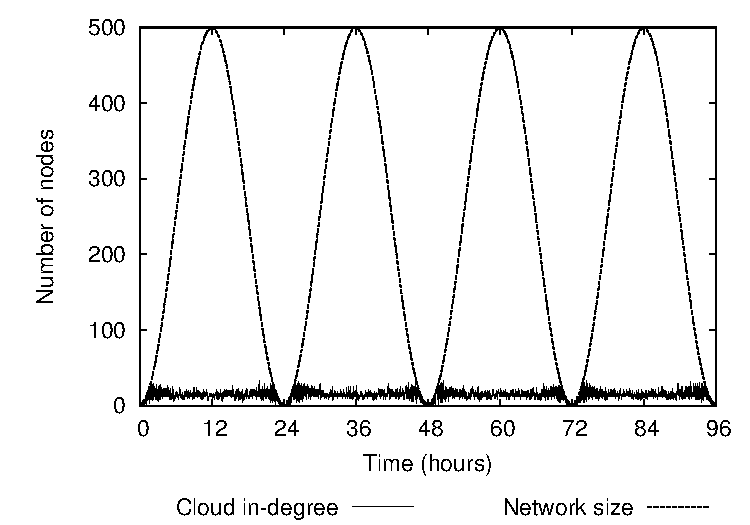
\includegraphics[width=240pt]{cloudcast-sim-oscillating-indegree.pdf}
    \label{fig:cloudcast-sim-oscillating-indegree}
  }
  \subfloat[][Detail of a simulated day]{
    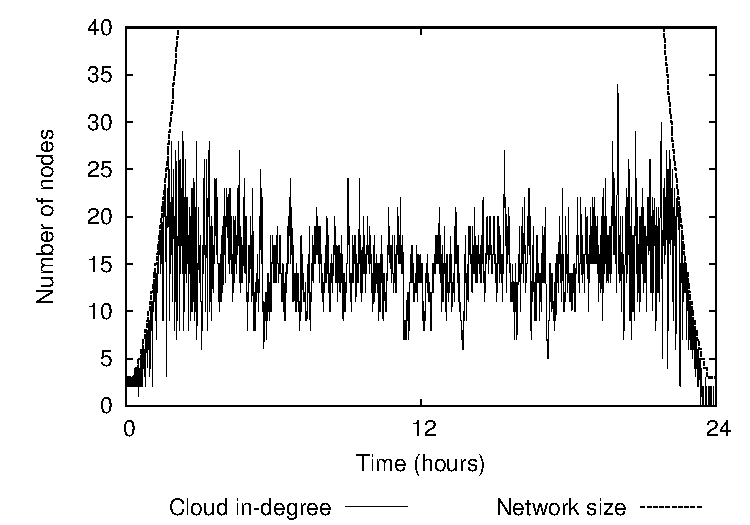
\includegraphics[width=240pt]{cloudcast-sim-oscillating-indegree-detail.pdf}
    \label{fig:cloudcast-sim-oscillating-indegree-detail}
  }
  \caption{\emph{Cloud} in-degree for a network oscillating daily
    between $0$ and $500$ nodes.}
  \label{fig:cloudcast-sim-oscillating-indegree-global}
\end{figure}

Moving our attention to the impact of the \peersampling protocol on
the \cloud, figure~\ref{fig:cloudcast-sim-loads} verifies the assertion
that the system scales well with the growing of the network size. The
plot relates the aggregated number of \cloud contacts, over the course
of the day, with different network sizes. As can be seen, small topologies
tend to relay for the most part on the \cloud, while the loads
decrease and stabilize for larger ones.

\begin{figure}[H]
  \centering
  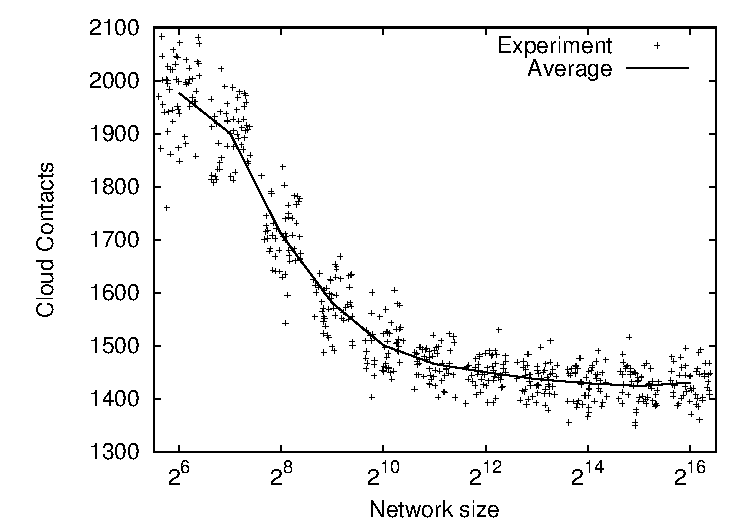
\includegraphics[width=.7\textwidth]{cloudcast-sim-loads.pdf}
  \caption{Storage \cloud load for different network sizes.}
  \label{fig:cloudcast-sim-loads}
\end{figure}

\subsection{Epidemic Broadcast}
For what concerns the \epidemic broadcast components of
\cloudcast, an interesting measurement is the delay with which peers
receive updates. This data is proposed in
figure~\ref{fig:cloudcast-sim-delays} for different network sizes.
Figure~\ref{fig:cloudcast-sim-oscillating-delays} instead keeps track
of the delays in a dynamic scenario of an oscillating network of
$500$ nodes. The dashed lines represent the average delay for each
update computed by the following rule: delta between the receiving
time of update $m$ by peer $i$ and the issuing time of update $m$, if
peer $i$ was active when update $m$ was issued; delta between the
receiving time of update $m$ by peer $i$ and the joining time of peer
$i$ otherwise.

\begin{figure}[H]
  \centering
  \subfloat[][Delays for different network sizes]{
    \hspace{-70pt}
    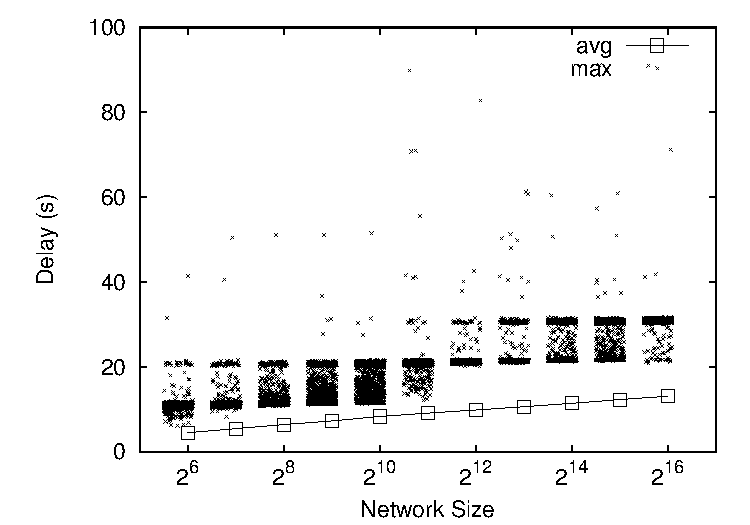
\includegraphics[width=240pt]{cloudcast-sim-delays.pdf}
    \label{fig:cloudcast-sim-delays}
  }
  \subfloat[][Progressive delays in a dynamic scenario]{
    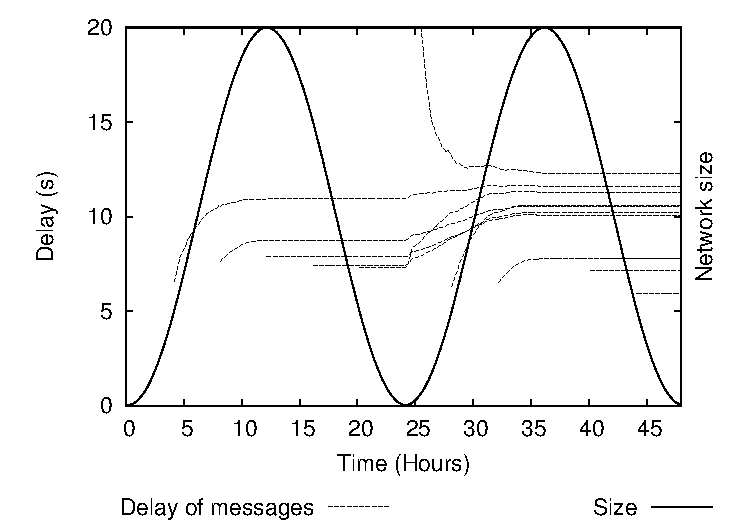
\includegraphics[width=240pt]{cloudcast-sim-oscillating-delays.pdf}
    \label{fig:cloudcast-sim-oscillating-delays}
  }
  \caption{Delays in messages diffusion for fixed and oscillating networks}
  \label{fig:cloudcast-sim-globa-delay}
\end{figure}

\section{Additions to the Peer Sampling protocol}
\label{sec:cloudcast-additions}
The results presented in the previous section prove that
\cloudcast is a stable protocol capable of forming and maintaining a
connected topology satisfying the constraints on the \cloud contact
rate. However,
the tricks that has been used by the simulation to emulate the interaction
with the storage service, hide some of the problem that real
implementations must face. For instance, in the real world, the
\cloud storage could be unreachable due to overload of the provider
or more realistically due to failure on the peer's end. Remembering
that peers selected as target in the active cycle are removed from the
local \view, this means that a temporary error contacting the
storage service could result in the loosing of all the
\cloud \descriptors in the network.

Even without considering this scenario, a recovery mechanism able to
re-establish the correct behavior is needed to guarantee the stability
of the protocol under any circumstance (e.g. abruptly removal of large
part of the topology).

To resolve this issue, during the course of this work, the
\peersampling protocol has been expanded with some minor additions.

% Insert additions cloudcast's protocol algorithms
\input algorithms/cloudcast_peersampling_algo_additions

Algorithm~\ref{algo:cloudcast_addition_active} shows the
supplementary actions performed by the modified \cyclon active thread,
while algorithm~\ref{algo:cloudcast_addition_passive} reports
the extra operations carried out by the passive routines.

Two variables have been added to reflect the new states of the protocol:
$bakC$, used to store a back-up copy of the \cloud \descriptor selected
as target, and $T$, which keeps track of the last time any peer
contacted the \cloud.

Blocks a1, a4 and a8 implement the safeguard on
\cloud entries. Whenever an active cycle involving the storage
service starts, the corresponding \cloud \descriptor is saved in the
variable $bakC$ (block a4). When the remote \view\ is received,
triggering the procedure responsible for the tuning of the
\cloud contact rate, the saved entry can be cleared, as the risk of
losing it is ceased (block a8). If, instead, the reply from the storage
service is not received in time for the next cycle, the saved entry is
reinstated (block a1). Since this check is done after the selection and
consequential removal of the target peer, it is guaranteed that the local
\view\ has a free spot for the backed-up \cloud \descriptor.

The next addition with respect to the original protocol regards the
recovery mechanism. In block a3 the variable $T$, containing the
timestamp of the last storage service contact, is tested against the
threshold parameter \maxsilence: in case of failure a new
\cloud entry is added to the local \view\ with probability
\spawnprob. The variable $T$ is updated every time the
\cloud is selected as target for the active cycle (block a4) and is
piggybacked on all the peers messages (blocks a5 and a6). When any
such message is received, the variable $T$ is confronted with the
remote counterpart and, if appropriate, updated (blocks a6 and a7).

Thanks to this strategy, if all the \cloud \descriptors are removed
from the topology, the ``black-out'' lasts for as much as
\maxsilence. The probabilistic insertion avoids a sudden explosion of
\cloud entries, while the usual tuning mechanism takes care of
restoring the optimal in-degree.

Block a2 concludes the analysis of the protocol's modifications. This
portion of pseudo code implements a simple check that forces the
addition of a \cloud entry in case of an empty \view. This simple
check is enough to guarantee that peers which remain cut off from the
topology can automatically rejoin the network.
